\documentclass[border=4pt]{standalone}
\usepackage{amsmath,amssymb,tikz}\usetikzlibrary{arrows.meta}
\definecolor{figB}{RGB}{31,90,166}\definecolor{figR}{RGB}{176,48,48}\definecolor{figG}{RGB}{46,125,50}\definecolor{figO}{RGB}{214,120,20}
\begin{document}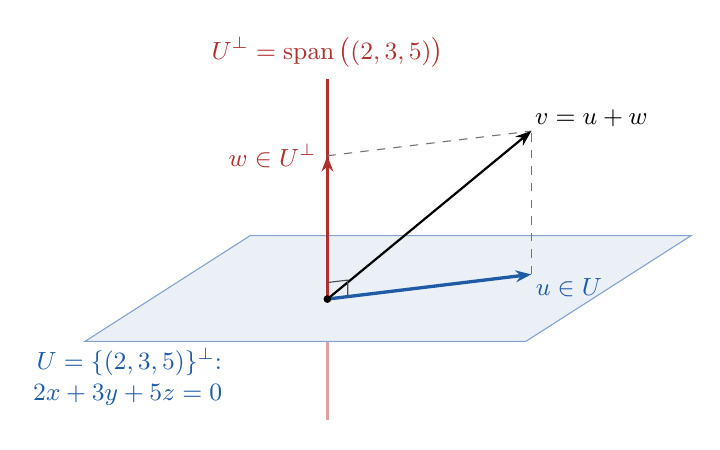
\begin{tikzpicture}[scale=1.4,>={Stealth[length=2mm]},x={(1cm,0cm)},y={(0.5cm,0.32cm)},z={(0cm,1cm)}]
% lower half of the line (behind the plane)
\draw[very thick,figR!45] (0,0,-1.1)--(0,0,0);
% the plane U
\fill[figB!9] (-1.6,-1.2,0)--(2.4,-1.2,0)--(2.4,1.8,0)--(-1.6,1.8,0)--cycle;
\draw[figB!55] (-1.6,-1.2,0)--(2.4,-1.2,0)--(2.4,1.8,0)--(-1.6,1.8,0)--cycle;
\node[figB,font=\small,anchor=north east,align=right,inner sep=2pt] at (-0.3,-1.2,0) {$U=\{(2,3,5)\}^\perp$:\\ $2x+3y+5z=0$};
% upper half of the line U-perp
\draw[very thick,figR] (0,0,0)--(0,0,2.0) node[above,font=\small]{$U^\perp=\operatorname{span}\big((2,3,5)\big)$};
% decomposition v = u + w
\coordinate (u) at (1.5,0.7,0); \coordinate (w) at (0,0,1.3); \coordinate (v) at (1.5,0.7,1.3);
\draw[dashed,black!55] (u)--(v); \draw[dashed,black!55] (w)--(v);
\draw[->,very thick,figB] (0,0,0)--(u) node[below right,font=\small,inner sep=1pt]{$u\in U$};
\draw[->,very thick,figR] (0,0,0)--(w) node[left,font=\small]{$w\in U^\perp$};
\draw[->,thick] (0,0,0)--(v) node[above right,font=\small,inner sep=1pt]{$v=u+w$};
\draw[black!70] (0,0,0.15)--++(0.15,0.07,0)--++(0,0,-0.15);
\fill (0,0,0) circle (1pt);
\end{tikzpicture}\end{document}
